\documentclass[a4paper]{article}

\usepackage[english]{babel}
\usepackage[utf8]{inputenc}
\usepackage{amsmath}
\usepackage{graphicx}
\usepackage[colorinlistoftodos]{todonotes}
\graphicspath{{./images/}}

\title{Traffic Light Detection with HOG Features and a Linear SVM}

\author{Daniel Engbert}

%\date{\today}
\date{May 20, 2018}

\begin{document}
\maketitle

\begin{abstract}
% Enter a short summary here. What topic do you want to investigate and why? What experiment did you perform?
    This paper investigates creating a computer vision model for identifying and labeling traffic lights.  HOG features were generated from 24x48 patches of training images and used to train a linear SVM.  The model was then retrained using the initial data set in combination with a set of false positives from the model when ran on samples from the training set.  The model is applied to test images using a gaussian pyramid and a sliding window.
% What were your main results and conclusion?
\end{abstract}

% Introduction/Background
\section{Introduction}
\label{sec:theory}
\subsection{Background}
The idea of self driving cars is becoming an increasingly more popular research topic as society seeks to reduce the number of traffic accidents by eliminating human error.  This topic is important because a functional self-driving car system has the potential to save thousands of lives once it is implemented.  One crucial element of a self driving car is the ability for it to recognize and read the state of traffic lights.

Histogram of Oriented Gradients (HOG) is an image feature that can be generated from an image and used to train a classifier.

% Explain the context of the experiment here
% Briefly explain what methods you will use in the experiment, and what values you will extract from the data.
%cite the Nano 3 Lecture notes \cite{nano3}.

\subsection{Related Work}
Omachi et al.\ presents a technique for detecting traffic lights ``taken from a single scene image taken from an in-vehicle camera'' \cite{omachi}.  Omachi et al.\ explain how template matching is a common techinque for detecting general objects, but it has a drawback of high computation complexity.  Their proposed technique is to detect filled circles in the image (of the same color as traffic lights) by normalizing and filtering the colors, then performing a Hough Transform \cite{omachi}.  Normalizing the colors is useful for providing robustness to lighting conditions which can vary due to factors such as time of the day and weather \cite{omachi}.

Charette et al.\ detected traffic lights by first performing spot light detection on the image in grayscale by looking for bright areas surrounded by darker area \cite{charette}.  Next they applied template matching to the remaining candidate regions using an ``Adaptive Template Matcher'' they designed that could be adjusted to represent traffic lights from desired countries.

Ji et al.\ detected red and green traffic lights using HOG features and an SVM classifier.  HOG features were generated from grayscale regions (resized to all be 15x30), and then a SVM was used to predict the class of the image.  The author's trained using features generated from patches of images known to contain traffic lights, and also with  patches known to not contain a traffic light.  The SVM classifier was then trained on the two classes ``positive'' and ``negative'' using the generated HOG features.  For detecting the state of a traffic light after the SVM model is ran, the bright and dark pixels within a positive region (believed to be a traffic light) are counted and used with their locations to predict the state of the traffic light.  The authors were able to process frames in an average of 143 ms, and the precesion and recall values for detecting red and green lights were all between 95.01\% and 97.55\% \cite{ji}.

Dalal et al.\ trained a linear SVM using HOG features to detect humans in images.  The authors demonstrated that by running the trained model again on the training images and saving the false positives, they could retrain the model on the initial data set combined with the false positives to ``significantly improve the performance'' of the model \cite{dalal}.  The authors also used evlauted images at mulitple scales (in a pyramid) to provide robustness to scale.

\section{Data Set}
The ``Bosch Small Traffic Lights Dataset'' is a set of 13,427 images at a resolution of 1280x720 pixels and contains 24,000 labeled traffic lights \cite{behrendt}.  The dataset is annoated with bounding boxes around each traffic light and contains the state of the light.

The data set is broken into a training set (5093 images containing 10,756 traffic lights) and a test set (8,334 consecutive images containing 13,486 traffic lights).

\subsection{Usage}
The data set contains the following label states for the training images:
\begin{itemize}
    \item Green: 5207 lights
    \item Yellow: 444 lights
    \item RedLeft: 1092 lights
    \item Red: 3057 lights
    \item GreenLeft: 178 lights
    \item off: 726 lights
    \item GreenRight: 13 lights
    \item GreenStraight: 20 lights
    \item GreenStraightRight: 3 lights
    \item RedRight: 5 lights
    \item RedStraight: 9 lights
    \item RedStraightLeft: 1 lights
    \item GreenStraightLeft: 1 lights
\end{itemize}
Due to the sample sizes of some of these categories, the model proposed in this paper will only use the following labels:
\begin{itemize}
    \item Green (containing all variations of green lights)
    \item Yellow
    \item Red (containing all variations of red lights)
    \item off
\end{itemize}
For training purposes, a label of ``other'' is also used to signify that a given image patch is not a traffic light.

\section{Proposed Method}
\subsection{Extracting Patches}
First we extract patches of images within the training set and save them along with their respective labels.  All traffic lights in the training set were extracted into unique patches, as well as about 15 random (non-traffic light) patches from each image to form the ``other'' set.

Each patch was resized to 24x48 prior to saving so that the HOG feature vector for each image would be the same size.  For each traffic light, the provided bounding box was widened or lengthened to have a 1:2 ratio, then the region was grown by a further 20\% to include more of its surroundings, and then finally scaled to 24x48.

\begin{figure}[!htb]
\centering
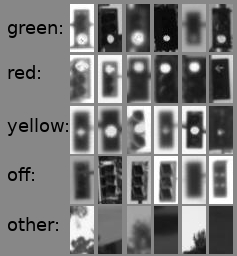
\includegraphics[width=0.5\textwidth]{trainingPatches.jpg}
    \caption{\label{fig:masks} Some of the samples from each class used for training}
\end{figure}

\subsection{HOG Features and SVM Training}
A HOG feature vector was then created for each image patch and stored along with the patch's label.  HOG was performed with 8x8 pixels per cell, and 9 orientation bins.  The image was also normalized using the power law before calculating the HOG.  Next a linear SVM was trained using the HOG feature vectors and their respective labels.

\subsection{Using the Model}
To apply the model to an image, a gaussian pyramid was used (for scale invariance) with the sliding window technique (with a step size of 5).  Regions with a non ``other'' label predicted with a confidence score of at least 95\% were kept.  After the sliding window was finished, non-maximum supression was applied to narrow down the detected regions.

\subsection{Retraining the Model}
After the model was trained initally (with the process above), it was ran on 200 images from the training set, and patches that were false positives were saved.  Then the model was retrained (as above) after the false positives were added to the set of extracted training patches under the label ``other''.
\subsubsection{False Positives}
%see figure \ref{fig:masks}.
\begin{figure}[!htb]
\centering
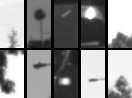
\includegraphics[width=0.5\textwidth]{falsePositives.jpg}
    \caption{\label{fig:masks} Some of the false positives}
\end{figure}
A lot of the false positives contained a circular shape that contrasted with the background.  Car tail lights were also common false positives.

\section{Testing and Results}
I tested my model on random images from the test data set (with a confidence threshold of 85\%).  After retraining with the false positives, the model made less predictions that were above the threshold and did not perform all that well.

 Below are the results when the model was applied to random images in the test set (using a confidence threshold of 85\%):
\begin{figure}[!htb]
\centering
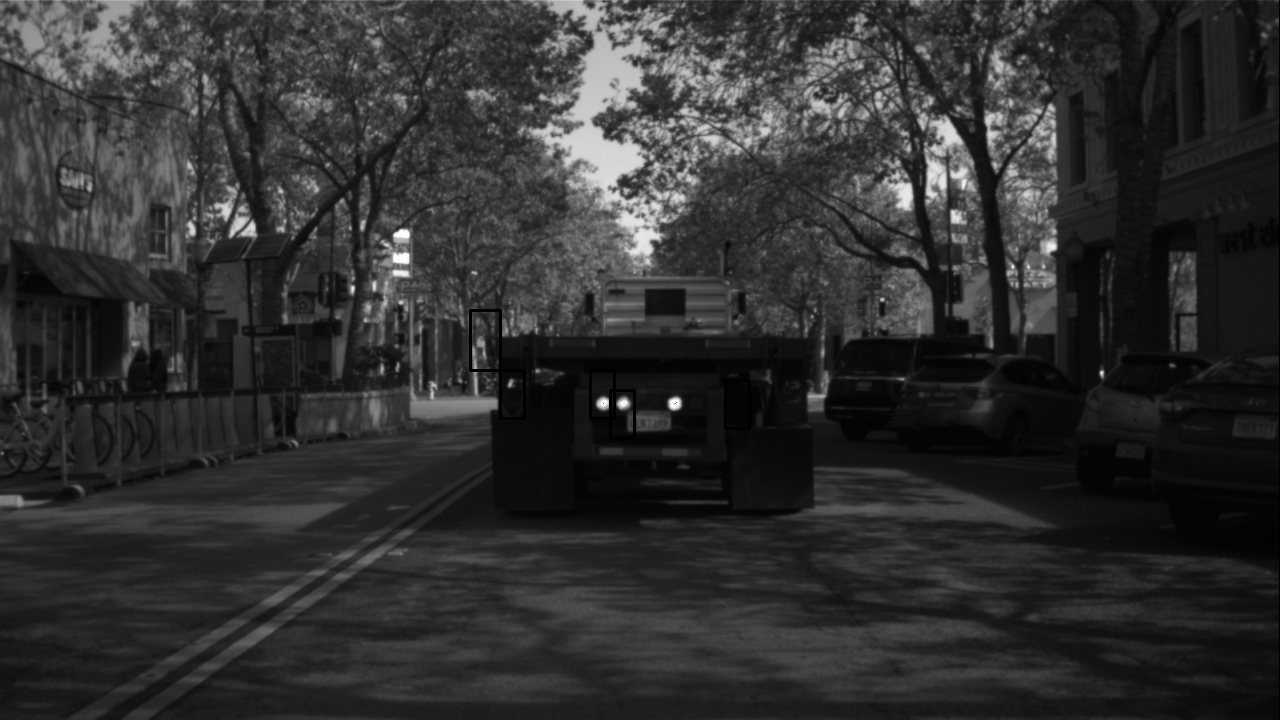
\includegraphics[width=0.4\textwidth]{25430.png}
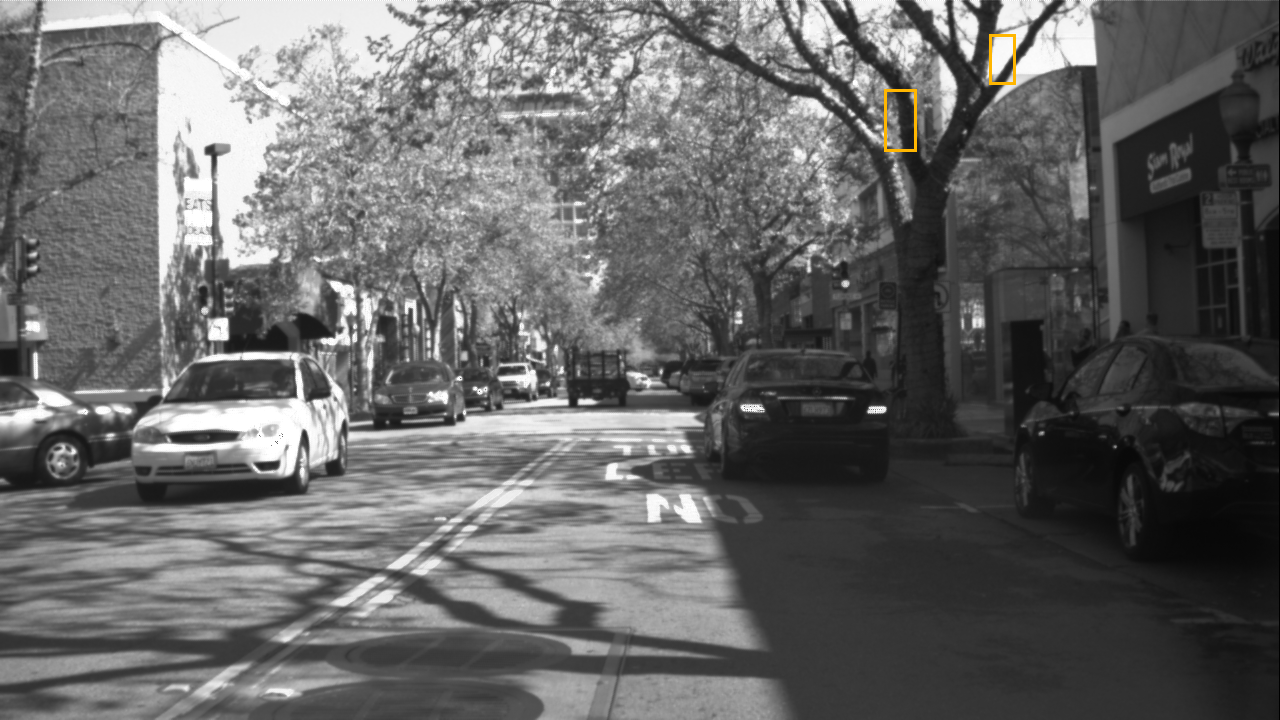
\includegraphics[width=0.4\textwidth]{28028.png}
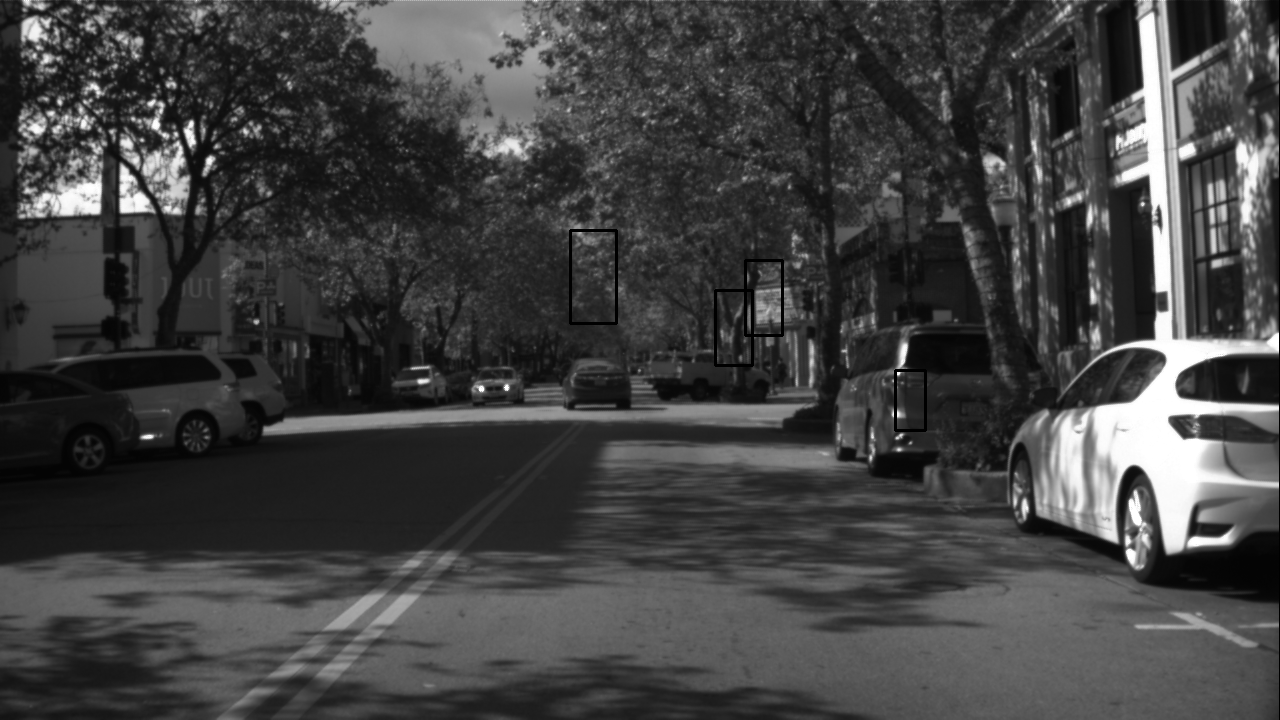
\includegraphics[width=0.4\textwidth]{38314.png}
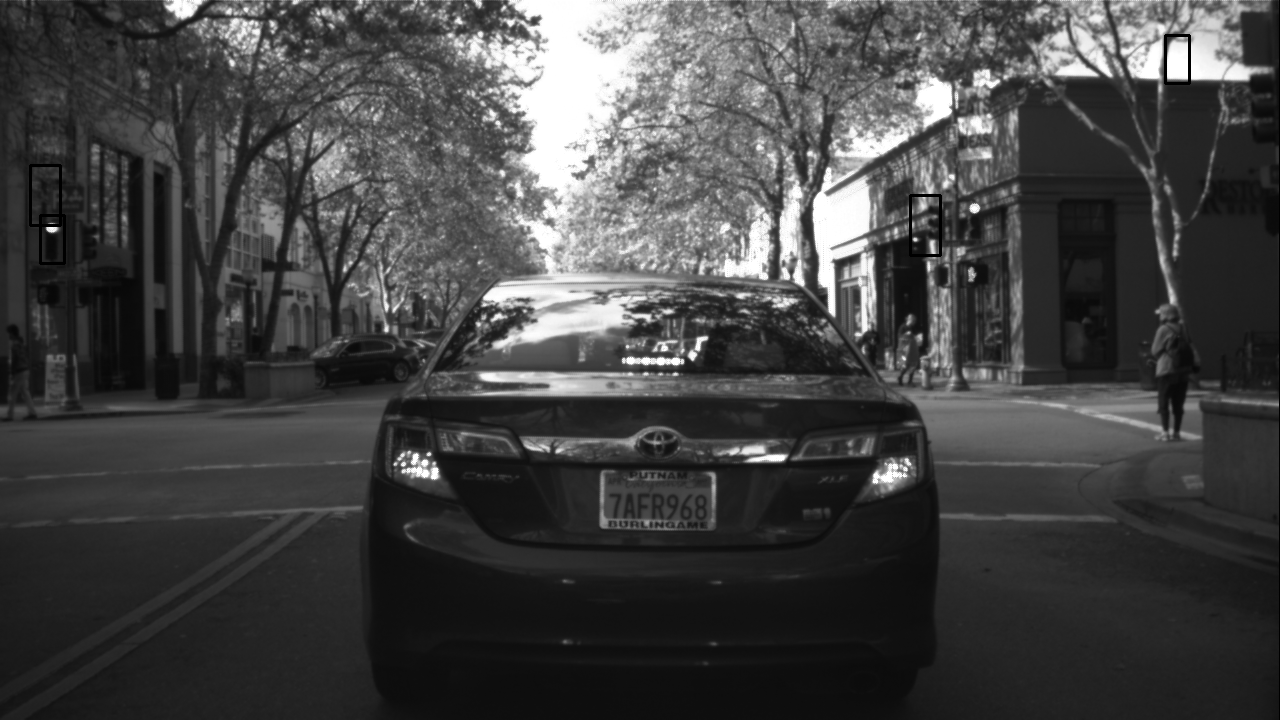
\includegraphics[width=0.4\textwidth]{37750.png}
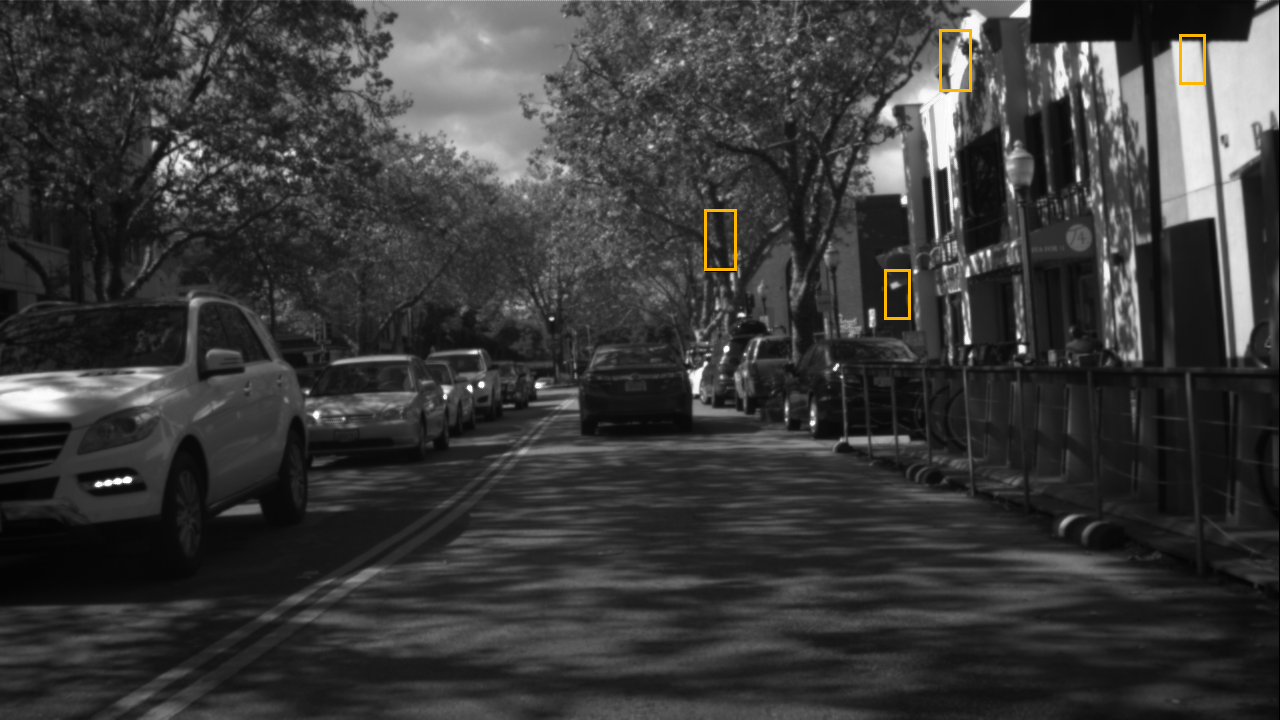
\includegraphics[width=0.4\textwidth]{39580.png}
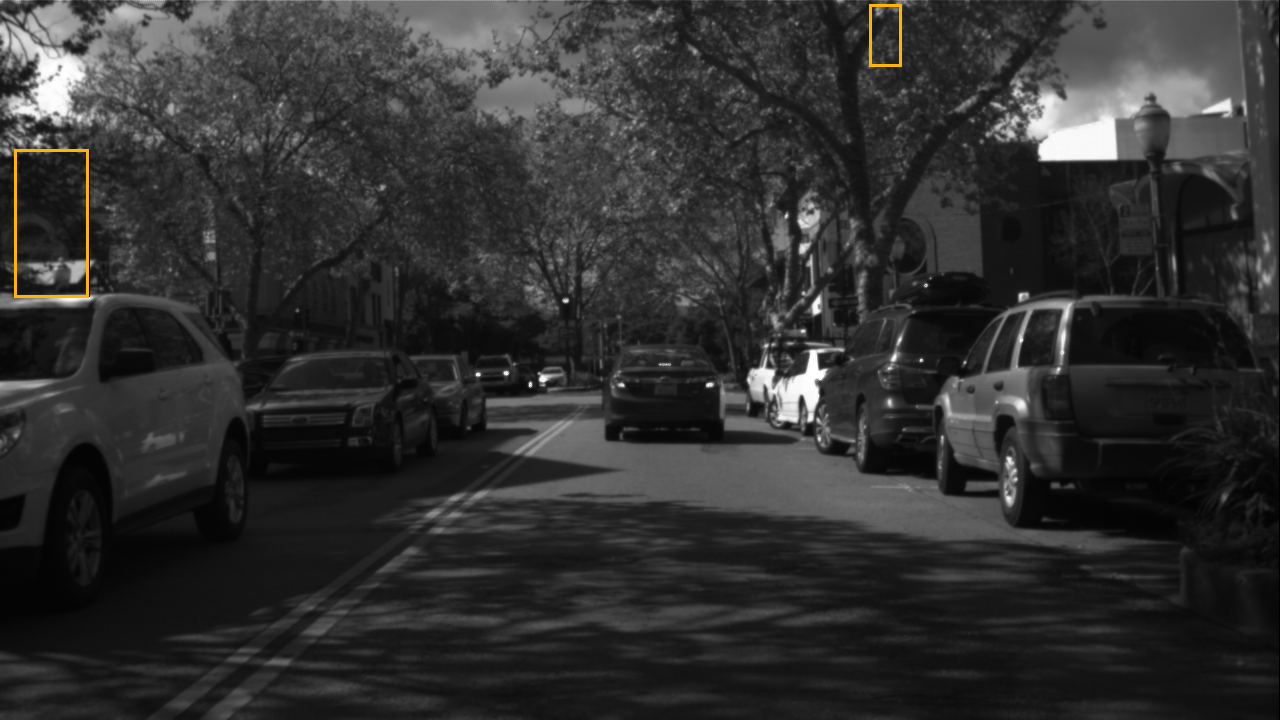
\includegraphics[width=0.4\textwidth]{39696.png}
    \caption{\label{fig:masks} Detected traffic lights are shown by a yellow border.}
\end{figure}


\subsection{Discussion and Conclusions}
The biggest issues with the model is that it is very slow to run on an image (takes about a minute).  Similar work by Ji et al.\ drasitically sped up there image processing by having a preprocessing step for detecting candidate regions, and then only considering those regions when generating HOG features \cite{ji}.  For future work it would be worth experimenting with a similar technique because having a slow detection time makes it harder to evaluate the model on sufficient quantity of test images.

One challenge with this dataset is that a lot of the traffic lights themselves are very small in the images, whereas with the pedestrian detector by Dalal et al., the humans were much bigger in the images.  Still I'm sure HOG and SVM could be tuned to gather better results than those seen here if I had more time. It would be interesting to cycle through training the model and adding false positives to the dataset numerous times rather than just performing this process once.


Note: The code used in this paper was adapted from https://github.com/bikz05/object-detector which used HOG and SIFT to detect cars within images.


\begin{thebibliography}{9}
\bibitem{behrendt}
    Behrendt, Karsten, Novak, \& Libor. (2017). Bosch Small Traffic Lights Dataset. Retrieved from https://hci.iwr.uni-heidelberg.de/node/6132/
\bibitem{charette}
    De Charette, R., \& Nashashibi, F. (2009, June). Real time visual traffic lights recognition based on spot light detection and adaptive traffic lights templates. In \emph{Intelligent Vehicles Symposium, 2009} IEEE (pp. 358-363). IEEE.
\bibitem{dalal}
    Dalal, N., \& Triggs, B. (2005, June). Histograms of oriented gradients for human detection. In Computer Vision and Pattern Recognition, 2005. CVPR 2005. IEEE Computer Society Conference on (Vol. 1, pp. 886-893). IEEE.
\bibitem{omachi}
    Omachi, M., \& Omachi, S. (2009, August). Traffic light detection with color and edge information. In \emph{Computer Science and Information Technology, 2009. ICCSIT 2009. 2nd IEEE International Conference on} (pp. 284-287). IEEE.
\bibitem{ji}
    Ji, Y., Yang, M., Lu, Z., \& Wang, C. (2015, June). Integrating visual selective attention model with HOG features for traffic light detection and recognition. In Intelligent Vehicles Symposium (IV), 2015 IEEE (pp. 280-285). IEEE.


\end{thebibliography}
\end{document}


% LATEX NOTES:::
% multiline comment
\iffalse
%\newpage
% see notes on creating tables and equations in original document
% creating tables
Use the table and tabular commands for basic tables --- see Table~\ref{tab:widgets}, for example.
\begin{table}
\centering
\begin{tabular}{l|r}
Item & Quantity \\\hline
Widgets & 42 \\
Gadgets & 13
\end{tabular}
\caption{\label{tab:widgets}An example table.}
\end{table}

% creating math equations
\LaTeX{} is great at typesetting mathematics. Let $X_1, X_2, \ldots, X_n$ be a sequence of independent and identically distributed random variables with $\text{E}[X_i] = \mu$ and $\text{Var}[X_i] = \sigma^2 < \infty$, and let

\begin{equation}
S_n = \frac{X_1 + X_2 + \cdots + X_n}{n}
      = \frac{1}{n}\sum_{i}^{n} X_i
\label{eq:sn}
\end{equation}

denote their mean. Then as $n$ approaches infinity, the random variables $\sqrt{n}(S_n - \mu)$ converge in distribution to a normal $\mathcal{N}(0, \sigma^2)$.
The equation \ref{eq:sn} is very nice.
\fi
